\documentclass{article}


\usepackage{mathtools}
\usepackage{listings}
\usepackage{enumitem}
\usepackage{fancyhdr}
\usepackage{extramarks}
\usepackage{amsmath}
\usepackage{amsthm}
\usepackage{amsfonts}
\usepackage{tikz}
\usepackage[plain]{algorithm}
\usepackage{algpseudocode}
\usepackage{graphicx}
\graphicspath{{images/}}
\usetikzlibrary{automata,positioning}

%
% Basic Document Settings
%

\topmargin=-0.45in
\evensidemargin=0in
\oddsidemargin=0in
\textwidth=6.5in
\textheight=9.0in
\headsep=0.25in

\linespread{1.1}

\pagestyle{fancy}
\lhead{\hmwkAuthorName}
\chead{\hmwkClass}
\rhead{\hmwkTitle}
\lfoot{\lastxmark}
\cfoot{\thepage}

\renewcommand\headrulewidth{0.4pt}
\renewcommand\footrulewidth{0.4pt}

\setlength\parindent{0pt}

%
% Create Problem Sections
%

\newcommand{\enterProblemHeader}[1]{
    \nobreak\extramarks{}{Problem \arabic{#1} continued on next page\ldots}\nobreak{}
    \nobreak\extramarks{Problem \arabic{#1} (continued)}{Problem \arabic{#1} continued on next page\ldots}\nobreak{}
}

\newcommand{\exitProblemHeader}[1]{
    \nobreak\extramarks{Problem \arabic{#1} (continued)}{Problem \arabic{#1} continued on next page\ldots}\nobreak{}
    \stepcounter{#1}
    \nobreak\extramarks{Problem \arabic{#1}}{}\nobreak{}
}

\setcounter{secnumdepth}{0}
\newcounter{partCounter}
\newcounter{homeworkProblemCounter}
\setcounter{homeworkProblemCounter}{1}
\nobreak\extramarks{Problem \arabic{homeworkProblemCounter}}{}\nobreak{}

%
% Homework Problem Environment
%
% This environment takes an optional argument. When given, it will adjust the
% problem counter. This is useful for when the problems given for your
% assignment aren't sequential. See the last 3 problems of this template for an
% example.
%
\newenvironment{homeworkProblem}[1][-1]{
    \ifnum#1>0
        \setcounter{homeworkProblemCounter}{#1}
    \fi
    \section{Problem \arabic{homeworkProblemCounter}}
    \setcounter{partCounter}{1}
    \enterProblemHeader{homeworkProblemCounter}
}{
    \exitProblemHeader{homeworkProblemCounter}
}

%
% Homework Details
%   - Title
%   - Due date
%   - Class
%   - Section/Time
%   - Instructor
%   - Author
%

\newcommand{\hmwkTitle}{Homework \#1}
\newcommand{\hmwkDueDate}{September 22, 2017}
\newcommand{\hmwkClass}{CSE 569 - Fundamentals of Statistical Learning}
\newcommand{\hmwkClassTime}{}
\newcommand{\hmwkClassInstructor}{Dr. Baoxin Li}
\newcommand{\hmwkAuthorName}{\textbf{Andrew Dudley}} 

%
% Title Page
%

\title{
    \vspace{2in}
    \textmd{\textbf{\hmwkClass:\ \hmwkTitle}}\\
    \normalsize\vspace{0.1in}\small{Due\ on\ \hmwkDueDate\ at 11:59pm}\\
    \vspace{0.1in}\large{\textit{\hmwkClassInstructor\ \hmwkClassTime}}
    \vspace{3in}
}

\author{\hmwkAuthorName}
\date{}

\renewcommand{\part}[1]{\textbf{\large Part \Alph{partCounter}}\stepcounter{partCounter}\\}

%
% Various Helper Commands
%

% Useful for algorithms
\newcommand{\alg}[1]{\textsc{\bfseries \footnotesize #1}}

% For derivatives
\newcommand{\deriv}[1]{\frac{\mathrm{d}}{\mathrm{d}x} (#1)}

% For partial derivatives
\newcommand{\pderiv}[2]{\frac{\partial}{\partial #1} (#2)}

% Integral dx
\newcommand{\dx}{\mathrm{d}x}

% Alias for the Solution section header
\newcommand{\solution}{\textbf{\large Solution}}

% Probability commands: Expectation, Variance, Covariance, Bias
\newcommand{\E}{\mathrm{E}}
\newcommand{\Var}{\mathrm{Var}}
\newcommand{\Cov}{\mathrm{Cov}}
\newcommand{\Bias}{\mathrm{Bias}}
\usepackage{color}
 
\definecolor{codegreen}{rgb}{0,0.6,0}
\definecolor{codegray}{rgb}{0.5,0.5,0.5}
\definecolor{codepurple}{rgb}{0.58,0,0.82}
\definecolor{backcolour}{rgb}{0.95,0.95,0.92}
 
\lstdefinestyle{mystyle}{
    backgroundcolor=\color{backcolour},   
    commentstyle=\color{codegreen},
    keywordstyle=\color{magenta},
    numberstyle=\tiny\color{codegray},
    stringstyle=\color{codepurple},
    basicstyle=\footnotesize,
    breakatwhitespace=false,         
    breaklines=true,                 
    captionpos=b,                    
    keepspaces=true,                 
    numbers=left,                    
    numbersep=5pt,                  
    showspaces=false,                
    showstringspaces=false,
    showtabs=false,                  
    tabsize=2
}
 
\lstset{style=mystyle}
\begin{document}
\maketitle
\thispagestyle{empty}
\pagebreak
\clearpage
\pagenumbering{arabic}
\begin{homeworkProblem}
    Consider the following decision rule for a two-category, one-dimensional problem:
    $$\text{Decide }\omega_1\text{ if  } x>0;\text{ otherwise, decide }\omega_2$$
    \begin{enumerate}[label=\alph*)]
        \item Show that the probabilty of error for this rule is given by $$P(\text{error})=P(\omega_1)\int_{-\infty}^\theta P(x|\omega_1)dx + P(\omega_2)\int_\theta^\infty P(x|\omega_2)dx$$
            \textbf{Solution}\\
            Given the decision rule, we know that there are two cases where we will incur error:
            \begin{enumerate}[label=(\arabic*)]
                \item $x < \theta \text{ when the  true state of nature is }\omega_1$
                \item $x \geq \theta \text{ when the  true state of nature is }\omega_2$
            \end{enumerate}
            Define $R_1=\{x\, |\, x > \theta\} \text{ and }$ $R_2=\{x\, |\, x \leq \theta\}$. 
            The probability of error for the decision rule can then be written as
            \begin{align}
                P(error)&=P(x\in R_2, \omega_1)+P(x\in R_1, \omega_2)\nonumber\\[0.5em]
                &=P(x\in R_2|\omega_1)P(\omega_1)+P(x\in R_1|\omega_2)P(\omega_2)\nonumber\\[0.5em]
                &=\int_{R_2}P(x|\omega_1)P(\omega_1)dx+\int_{R_1}P(x|\omega_2)P(\omega_2)dx\nonumber\\[0.5em]
                &=P(\omega_1)\int_{R_2}P(x|\omega_1)dx+P(\omega_2)\int_{R_1}P(x|\omega_2)dx\nonumber\\[0.5em]
                & \boldsymbol{ \color{blue}=P(\omega_1)\int_{-\infty}^\theta P(x|\omega_1)dx + P(\omega_2)\int_\theta^\infty P(x|\omega_2)dx\nonumber }
            \end{align}
        \item By differentiating, show that a necessary condition to minimize P(error) is that $\theta$ satisfy
            $$P(\theta\, |\, \omega_1)P(\omega_1) = p(\theta\, |\, \omega_2)P(\omega_2)$$
            \textbf{Solution}\\
            Using Leibniz' Integral Rule,
            $$\frac{d}{d\theta}\left [P(\omega_1)\int_{-\infty}^\theta P(x|\omega_1)dx + P(\omega_2)\int_\theta^\infty P(x|\omega_2)dx\right ]$$
            \begin{align*}
                =\;&P(\omega_1)\left [ \int_a^\infty \frac{\delta}{\delta\theta}[P(x\, |\, \omega_1)]dx + P(\omega\, |\, \omega_1)\cdot\frac{d}{d\theta}\theta-P(a\, |\, \omega_1)\cdot\frac{d}{d\theta}a\right ] \\[0.5em]
                &+P(\omega_2)\left [ \int_\theta^b \frac{\delta}{\delta\theta}[P(x\, |\, \omega_2)]dx + P(\omega\, |\, \omega_1)\cdot\frac{d}{d\theta}\theta-P(a\, |\, \omega_1)\cdot\frac{d}{d\theta}a\right ]\\[0.5em]
              =\;&P(\theta\, |\, \omega_1)P(\omega_1) - p(\theta\, |\, \omega_2)P(\omega_2)
            \end{align*}
            To minimize P(error), we will need a mininum value of the function, and the rate of change of P(error) at that point will be 0.
            $$P(\theta\, |\, \omega_1)P(\omega_1) - p(\theta\, |\, \omega_2)P(\omega_2)= 0$$
            which gives us
            $$\color{blue}\mathbf{P(\theta\, |\, \omega_1)P(\omega_1) = p(\theta\, |\, \omega_2)P(\omega_2)}\text{.}$$
        \item Does this equation satisfy $\theta$ uniquely?
            \\\textbf{Solution}\\
            No. If the class conditional probability density functions intersect more than once - resulting in disjoint regions - then there will be multiple values of theta that satisfy the criterion
            $$P(\theta\, |\, \omega_1)P(\omega_1) - p(\theta\, |\, \omega_2)P(\omega_2)= 0$$
        \item Give an example where a value of $\theta$ satisfying the equation actually maximizes the probability of error. \\
            \textbf{Solution}\\
            If the class-conditional probability density distributions for $\omega_1$ and $\omega_2$ are Gaussian and the mean of the gaussian distribution for $\omega_1$ is less than the mean for $\omega_2$, then $\theta$ will maximize the probability of error.
    \end{enumerate}

\end{homeworkProblem}
\begin{homeworkProblem}
    Consider a one-dimensional, two-category classification problem, with equal prior probabilities $(P(\omega_1)=P(\omega_2)=\frac{1}{2})$. The class-conditional PDFs for the two classes are the normal densities $N(\mu_1,\sigma^2)$ and $N(\mu_2,\sigma^2)$, respectively. Note that these two PDFs have the same variance $\sigma^2$. $N(\mu, \sigma^2)$ denotes the normal density defines by
    $$p(x\, |\, \mu) = \frac{1}{\sqrt{2\pi}\sigma}e^{-\frac{(x-\mu)^2}{2\sigma^2}}\text{.}$$
    We further assume that the losses $\lambda_{11}=\lambda_{22}=0$, but $\lambda_{12}$ and $\lambda_{21}$ are non-zero.
    Find the optimal decision rule for classifying any feature point x.\\
    \textbf{Solution}\\
    In general, a two-category classification problem reduces to the Bayes decision rule:
    $$\text{Decide }\omega_1\text{ if  } (\lambda_{21}-\lambda_{11})p(x\, | \, \omega_1)P(\omega_1)>(\lambda_{12}-\lambda_{22})p(x\, | \, \omega_2)P(\omega_2)\text{; otherwise, decide }\omega_2$$
    Because of the equal variance and equal prior probabilities, the equation of the decision rule reduces to 
    \begin{align*}
        &&ln(\lambda_{21})+(-[x^2-2x\mu_1+\mu_1^2]) \,&>\, ln(\lambda_{12})+(-[x^2-2x\mu_2+\mu_2^2])\\
        \Longrightarrow&&2x\mu_1-2x\mu_2\,&\,>-\mu_2^2+\mu_1^2+ln\left (\frac{\lambda_{12}}{\lambda_{21}}\right )\\
    \end{align*}
    We can define the region $R_1$ by solving for x
    $$\mathbf{R_1=\left \{x \, \left | \, x<\frac{\mu_2^2+\mu_1^2+ln\left (\frac{\lambda_{12}}{\lambda_{21}}\right )}{2(\mu_2-\mu_1)}\right . \right \}}$$
    Which results in the optimal decision boundary
    $$\mathbf{\textbf{Decide }\omega_1\text{ if  } x \in R_1\textbf{; otherwise, decide }\omega_2}$$
\end{homeworkProblem}
\begin{homeworkProblem}
Consider a two-class classification problem with one-dimensional class-conditionals given as
$$P(x\, | \, \omega_1) = \frac{1}{\sqrt{2\pi}}e^{-\frac{(x-1)^2}{2}}\text{,}$$
$$P(x\, | \, \omega_2) = \begin{cases}
    \frac{1}{3}, \text{ if } 0\leq x\leq 3\\
    0, \text{ otherwise}
    \end{cases}$$
    Suppose the priors are $P(\omega_1)=\frac{2}{3}, P(\omega_2)=\frac{1}{3}$. Find the optimal decision rule for doing the classification. What is the Bayes error in this case?\\
    \textbf{Solution}\\
    Given that the class-conditional PDF for $\omega_1$ is a Guassian distribution and the PDF for $\omega_2$ is a simple geometric shape, we can solve this problem geometrically. 

    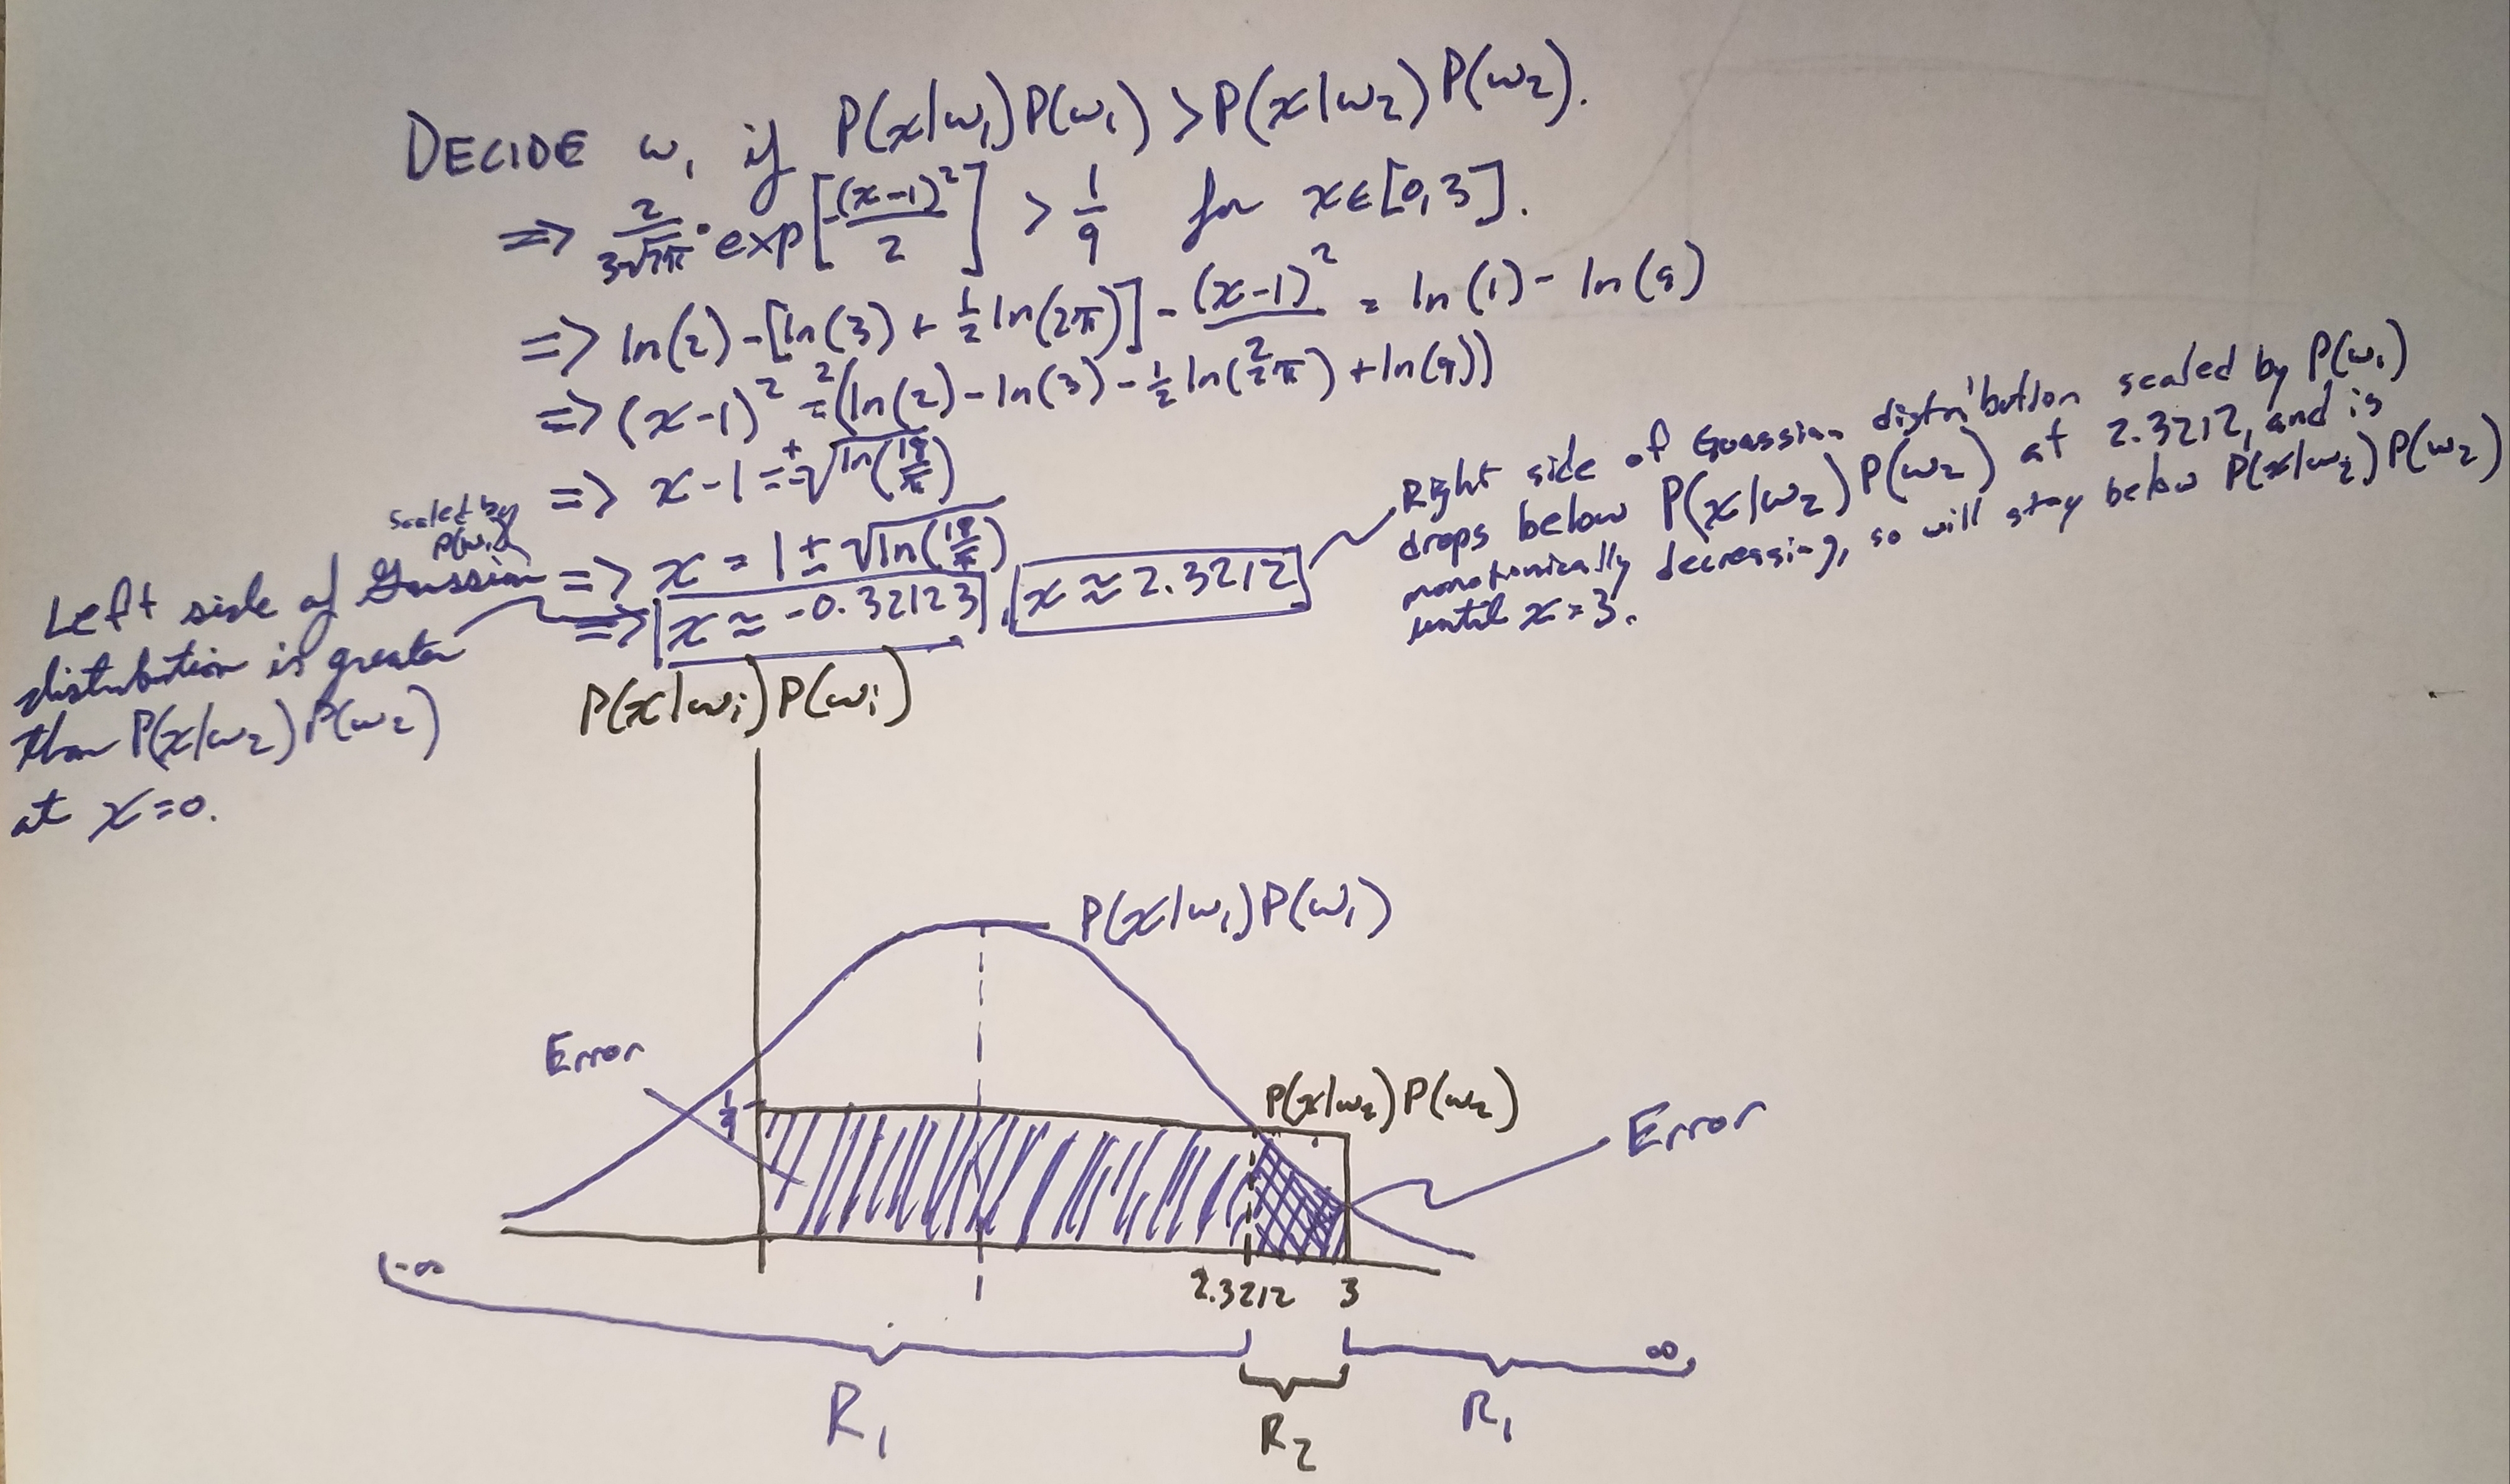
\includegraphics[width=0.75\linewidth]{p3_image_2.jpg}\\
    $P(x|\omega_1)P(\omega_1)$ (the posterior probability scaled by $p(x)$) intersects the line $y=1/9$ at two points, once at $x = -0.32123$ (which outside of the domain of $P(x|\omega_2)$) and once at $x\approx 2.3212$. This tells us that the region where $P(\omega_1\, |\, x) > P(\omega_2\, |\, x)$ can be defined as 
    $$\mathbf{ R_1 = \{x\, |\, x < 2.3212 \text{ or } x > 3\} }$$
    
    This problem has a zero-one loss function, so the conditional risk can be calculated as
    $$R(\alpha_i\, |\, x)=1-P(\omega_i\, |\, x)$$

    and the Bayes Rules to minimize risk says to minimize the conditional risk, so we choose the value of $i$ that maximizes $P(\omega_i\, |\, x)$, leading us to the decision rule
    $$\mathbf{ \textbf{Decide }\omega_1\textbf{ if } x \in R_1 \textbf{; otherwise, decide }\omega_2}$$

    The Bayes error can be calculated with the formula
    $$P(error)=P(\omega_1)\int_{R_2}P(x|\omega_1)dx+P(\omega_2)\int_{R_1}P(x|\omega_2)dx$$
    Worked out below\dots\\
    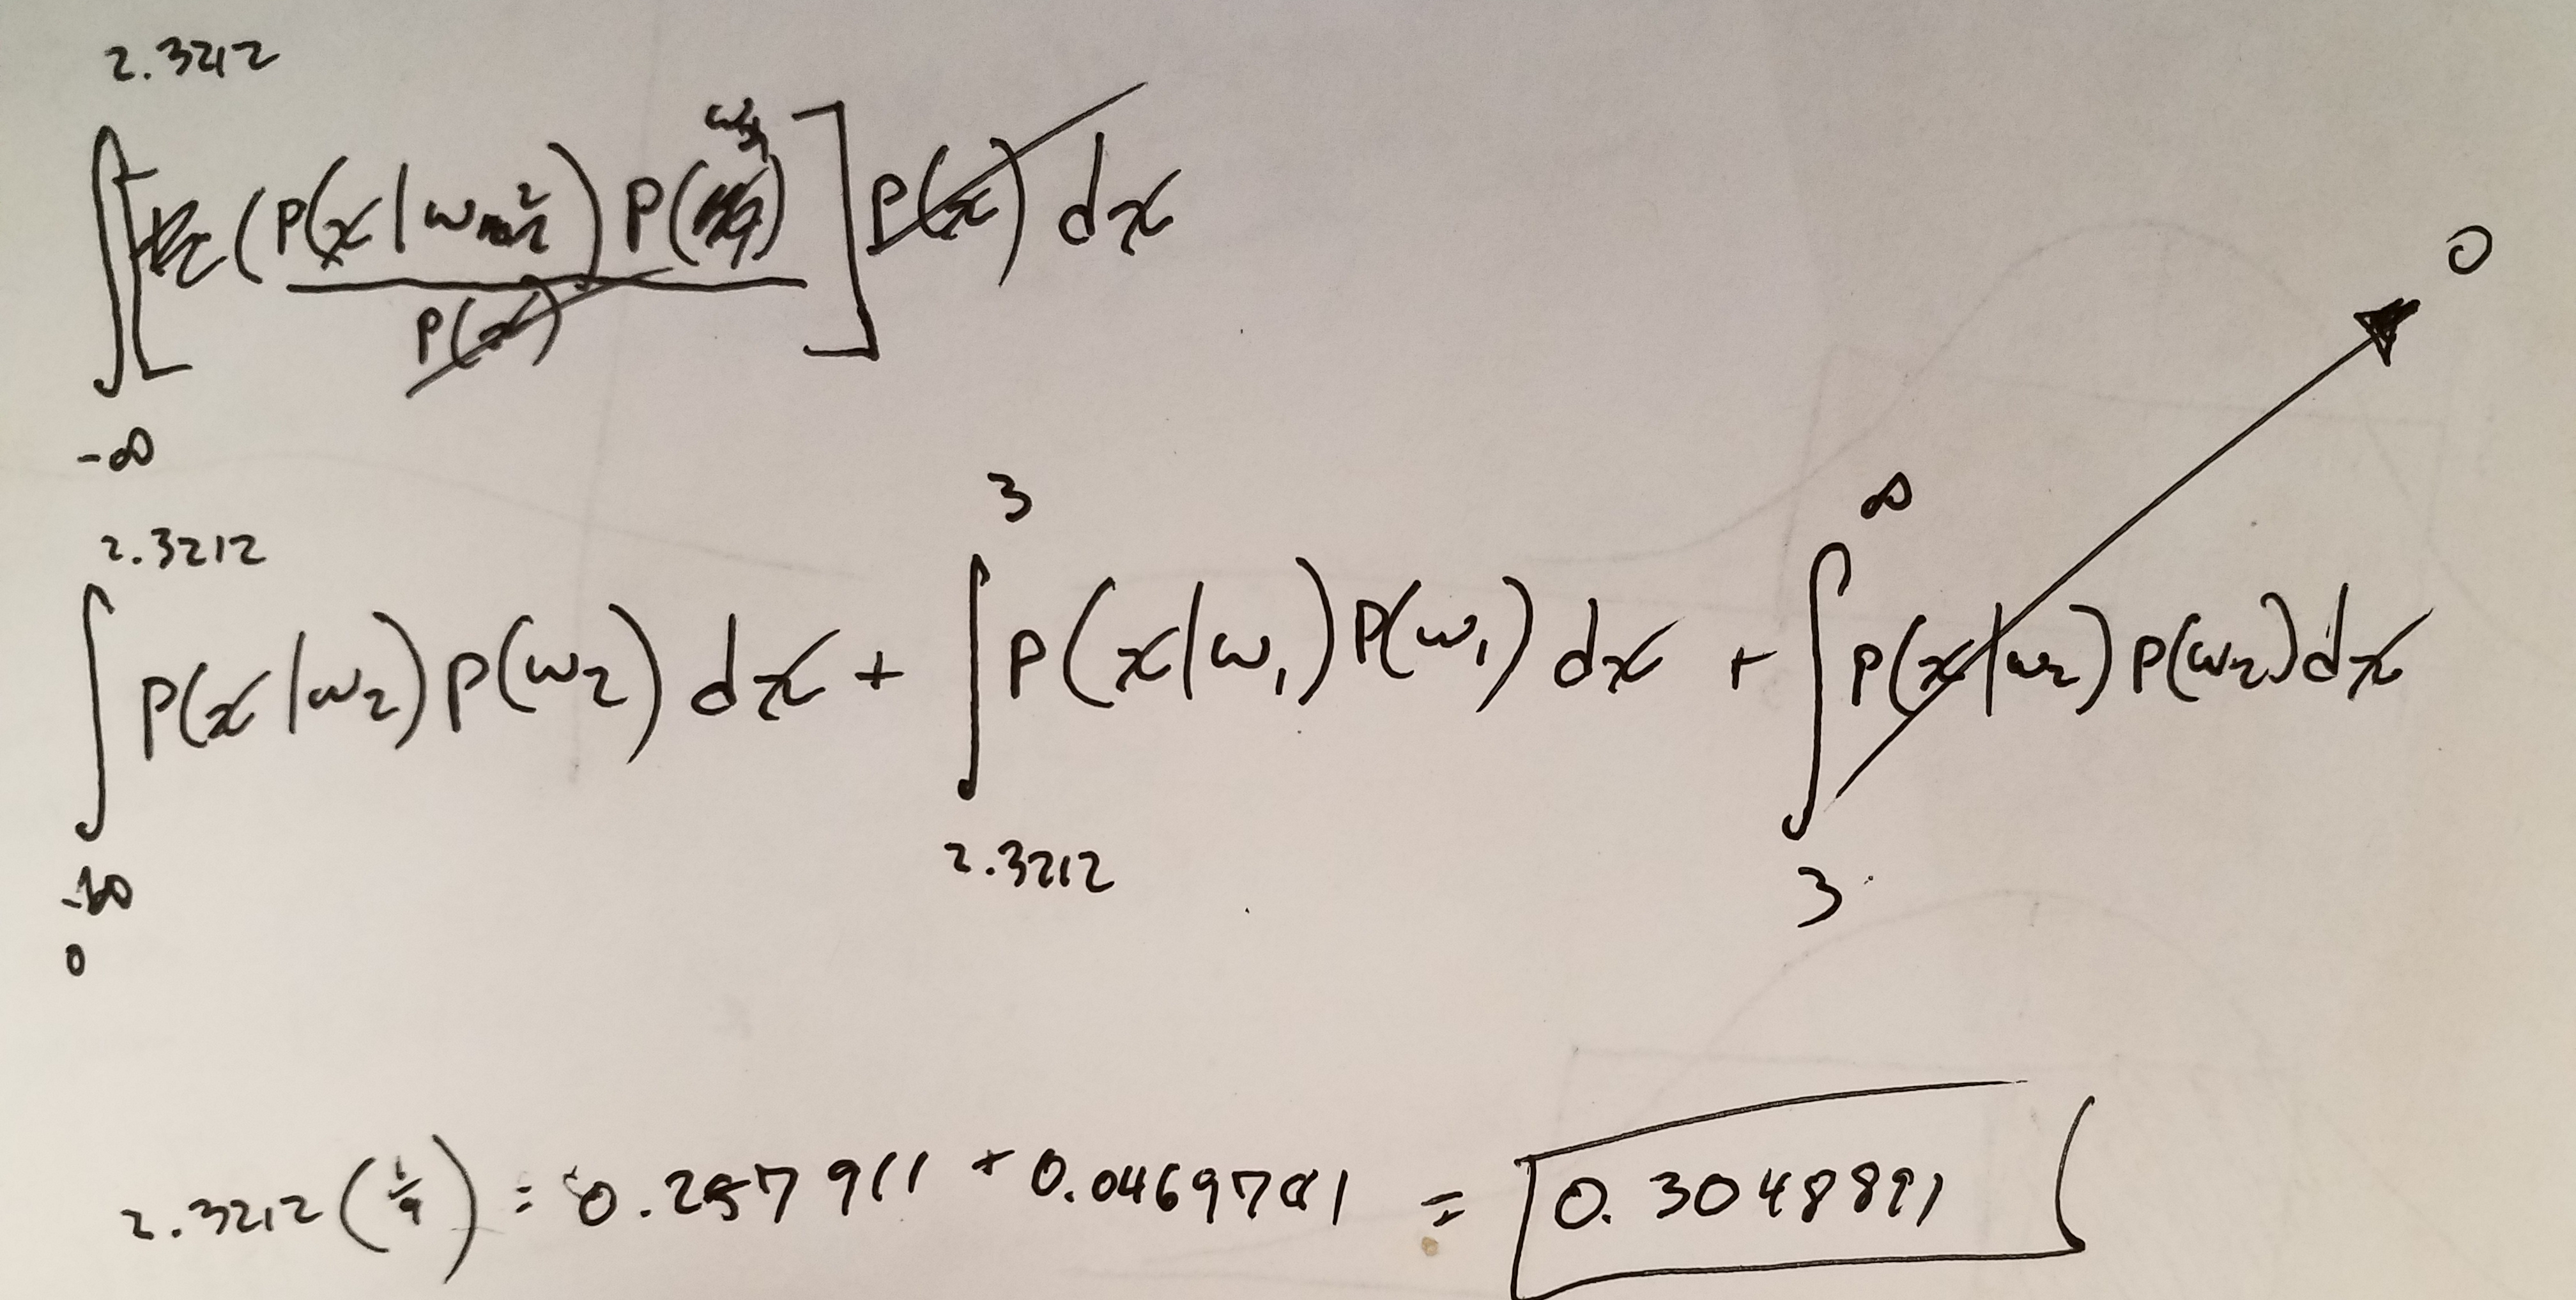
\includegraphics[width=0.75\linewidth]{p3_image.jpg}\\
    Therefore, $\mathbf{P(error)\approx 0.30489}$
    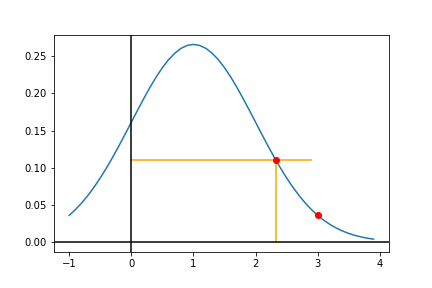
\includegraphics[width=0.5\linewidth]{plot.png}\\

\end{homeworkProblem}
\begin{homeworkProblem}
    Consider the following Bayesian network where all of the nodes are assigned to be binary random variables
    \begin{enumerate}[label=\alph*)]
    \item Suppose that X is measured and its value is $x_1$, compute the probability that we will observe W having a value $\omega_1$. i.e., $P(\omega_0\, | \, x_1)$

    \textbf{Solution}\\
    Need the marginalized probability of $\omega_0$ conditioned on $x_1$.
    \begin{align*}
        P(\omega_0 \, | x_1) &= p(x_1)\frac{\sum_Y \sum_Z P(Y\, |\, x_1)P(Z \, | \, Y)P(w_0\, |\, Z)}{p(x_1)}\\[0.5em]
        &= \sum_Y P(Y\, |\, x_1)\sum_Z P(Z \, | \, Y)P(w_0\, |\, Z)\\
        &= 0.6(0.4(0.7) + 0.6(0.55)) + 0.4(0.75(0.7) + 0.25(0.55))\\
        &\mathbf{= 0.631}
    \end{align*}
    \item Suppose that W is measured and its value is $w_1$, compute the probability that we will observe X having a value $x_0$.
        \begin{align*}
            P(x_0\, |\, w_1) &= \frac{P(x_0, w_1)}{P(w_1)}\\
            &= \frac{\sum_Y \sum_Z P(x_0)P(Y\, | \, x_0)P(Z\, | \, Y)P(w_1\, | \, Z)}{\sum_X \sum_Y \sum_Z P(X)P(Y\, | \, X ) P(Z \, |\,  Y)P(w_1\, | \, Z)}\\[.5em]
            &= \frac{P(x_0)\sum_Y P(Y\, | \, x_0)\sum_Z P(Z\, | \, Y)P(w_1\, | \, Z)}{\sum_X P(X) \sum_Y P(Y\, | \, X )\sum_Z P(Z\, | \, Y) P(w_1\, | \, Z)}\\[.5em]
            &= \dfrac{0.4[0.7(0.4*0.3+0.6*0.45)+0.3(0.75*0.3+0.25*0.45)]}{\splitdfrac{0.4[0.7(0.4*0.3+0.6*0.45)+0.3(0.75*0.3+0.25*0.45)]}{ + 0.6[0.6(0.4*0.3+0.6*0.45)+0.4(0.75*0.3+0.25*0.45)]}}\\[.5em]
            &= 0.403395
        \end{align*}
    \end{enumerate}
\end{homeworkProblem}
\begin{homeworkProblem}
    True or False: For a two-class classification problem using the minimum-error-rate rule, in general the decision boundary can take any form. However, if the underlying class-conditionals are Gaussian densities, then the decision boundary is linear (hyperplanes).

    \textbf{Solution}\\
    False. If the covariance matrices for the Gaussian class-conditional PDFs are different, the disriminant function will be 
    $$g_i(x)=\mathbf{x^t W_i x}+\mathbf{W_i x}+w_{i0}$$
    where
    $\mathbf{x^t W_i x}$
    is inherently quadratic.
\end{homeworkProblem}
\begin{homeworkProblem}
    \begin{enumerate}[label=\alph*)]
    \item Consider the following game: Someone shows you three hats and tells you that there is a prize in one of them. He asks you to choose one of the hats. You choose one hat and tell him which one you chose. He then lifts one of the hats you didn't choose and there is nothing under that hat. He then tells you that you can either stay with the hat you have originally chosen or switch to the other remaining hat. What should you do? Explain your answer.
    
    \textbf{Solution}\\
    You should always switch.

    Intuitively, after you have chosen a hat there are two possible outcomes: 1/3 of the time, you will choose correctly, in which case the carnie can choose either of the remaining hats to lift. 2/3 of the time, you will choose wrong, in which case the carnie will be forced to lift the hat that doesn't contain the prize (inherently pointing out the hat that \textit{does} have the prize).

    \textbf{Bayes Rule proof:}\\
    A priori, $P(h_1)=P(h_2)=P(h_3)=1/3$ where $P(h_i)$ is the prior probability that the prize is under hat i.\\
    Assume we choose hat 1. The carnie knows which hat the prize is under, so we can calculate the class-conditional probability mass functions for the observations $D$ that the carnie chooses to flip hat 2 or hat 3.
    \begin{align*}
        P(d_2\, | \, h_1) = \frac{1}{2} && P(d_3\, | \, h_1) = \frac{1}{2}\\
        P(d_2\, | \, h_2) = 0 && P(d_3\, | \, h_2) = 1\\
        P(d_2\, | \, h_3) = 1 && P(d_3\, | \, h_3) = 0\\
    \end{align*}
    From the Bayes Rule, we know that 
    $$P(H\, |\, D)=\frac{P(D\,|\,H)P(H)}{\sum_H P(D\,|\,H)P(H)}$$
    So the posteriors can be calculated as:
    \begin{align*}
        P(h_1\,|\,d_2) &&= \frac{P(d_2\, | \, h_1)P(h_1)}{\sum_H P(d_2\, |\, H)P(H)} &= \frac{\frac{1}{2}*\frac{1}{3}}{\frac{1}{2}*\frac{1}{3}+0*\frac{1}{3}+1*\frac{1}{3}} &&= \frac{1}{3}\\
        P(h_2\,|\,d_2) &&= \frac{P(d_2\, | \, h_2)P(h_2)}{\sum_H P(d_2\, |\, H)P(H)} &= \frac{0*\frac{1}{3}}{\frac{1}{2}*\frac{1}{3}+0*\frac{1}{3}+1*\frac{1}{3}} &&= 0\\
        P(h_3\,|\,d_2) &&= \frac{P(d_2\, | \, h_3)P(h_3)}{\sum_H P(d_2\, |\, H)P(H)} &= \frac{1*\frac{1}{3}}{\frac{1}{2}*\frac{1}{3}+0*\frac{1}{3}+1*\frac{1}{3}} &&= \frac{2}{3}\\[1em]
        P(h_1\,|\,d_3) &&= \frac{P(d_3\, | \, h_1)P(h_1)}{\sum_H P(d_3\, |\, H)P(H)} &= \frac{\frac{1}{2}*\frac{1}{3}}{\frac{1}{2}*\frac{1}{3}+1*\frac{1}{3}+0*\frac{1}{3}} &&= \frac{1}{3}\\
        P(h_2\,|\,d_3) &&= \frac{P(d_3\, | \, h_2)P(h_2)}{\sum_H P(d_3\, |\, H)P(H)} &= \frac{0*\frac{1}{3}}{\frac{1}{2}*\frac{1}{3}+1*\frac{1}{3}+0*\frac{1}{3}} &&= \frac{2}{3}\\
        P(h_3\,|\,d_3) &&= \frac{P(d_3\, | \, h_3)P(h_3)}{\sum_H P(d_3\, |\, H)P(H)} &= \frac{1*\frac{1}{3}}{\frac{1}{2}*\frac{1}{3}+1*\frac{1}{3}+0*\frac{1}{3}} &&= 0
    \end{align*}
    Clearly, regardless of which hat the carnie flips, it is always in our best interest to switch.
    \item Design a computer-based experiment to simulate the above game to verify your answer, by playing the game many times to obtain an averaged performance.

        \textbf{Results}\\
        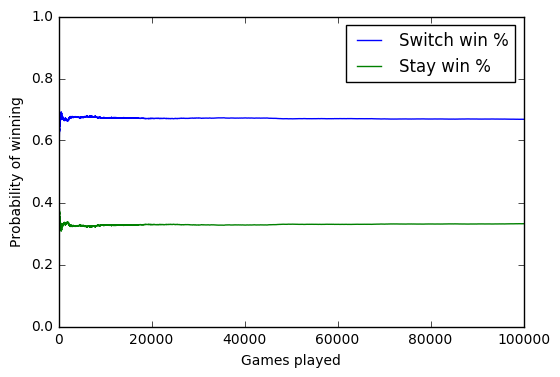
\includegraphics[]{results.png}
        \\
        \textbf{Code}\\
        \lstinputlisting[language=Python]{code.py}
\end{enumerate}

\end{homeworkProblem}
\end{document}
